\chapter{Join Process \\
  \small{\textit{-- Evan Ciok, Sophia DiCuffa, Carson McManus}}
  \index{Chapter!join-process}
  \index{join process}
  \index{room join}
  \label{Chapter::JoinProcess}}

There are 2 types of nodes in this architecture. The first type is the OTT Monolith \index{monolith}, which refers to the current node.js monolithic server. The second type is the Smart Load Balancer \index{load balancer}, which needs to know which monoliths control which rooms, and how to route requests to the correct monolith.

For the sake of simplicity, the initial implementation of the Balancer will be a single node. This can be upgraded to a cluster of load balancers in the future.


TODO: describe the room join process
TODO: be sure to talk about how clients are authorized

\section{Joining a Loaded Room \index{loaded room}}

In the Monolith, "loading" a room is literally creating an instance of a room in memory.

Shown in figure \ref{Figure::join-room-happy-path}, the client is joining a room that is already loaded on a Monolith node. First, the client initiates a websocket \index{websocket} connection to the Balancer, in the form of a HTTP request with the CONNECT method. The client immediately sends an "auth" message to convey their identity to the Balancer. The Balancer looks at the path of the request and extracts the room name, and references it's internal hashmap to find the monolith that is hosting the room. The Balancer then opens a websocket connection using the auth token provided by the client.

If the client fails to provide an auth token, the Balancer must terminate the connection as "timed out".

\begin{figure}[!htb]
  \centering
  \scalebox{0.57}{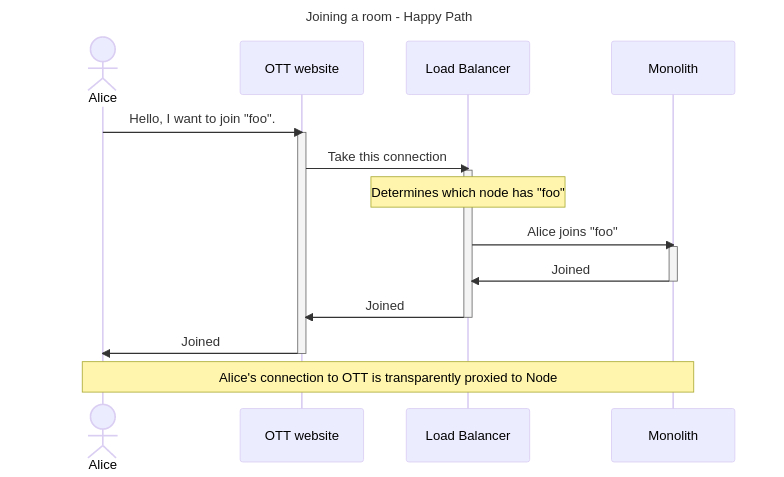
\includegraphics{Figures/join-room-happy-path.png}}
  \caption{\label{Figure::join-room-happy-path} Joining an already loaded room, the most simple scenario.}
\end{figure}

\subsection{Monolith Gossip Protocol \index{Monolith} \index{gossip}}

Balancers must be able to determine which Monolith nodes are hosting which rooms.

Monolith nodes must gossip \cite{wikigossip} \index{gossip} to Balancer nodes to inform them of the rooms that they have loaded. This also implies that they must notify all Balancers of their existance on startup. The Balancer must maintain a hashmap of room names to Monolith nodes.

They must also maintain a hashmap of monolith nodes to a list of rooms that they are hosting to verify that only one monolith is hosting a room at a time. When the gossip is received, the Balancer must check to see if  In the event that a Balancer finds that more than one Monolith is hosting a room, it must randomly select one of the Monoliths to be the authoritative node for that room, and inform the other Monoliths that they must unload the room. This method will not work as effectively if there is more than one Balancer, but it is a simple solution for the initial implementation.

Monoliths must gossip:
\begin{itemize}
  \item on startup
  \item when a room is loaded
  \item when a room is unloaded
  \item at a maximum interval of 20 seconds (eg. if 20 seconds pass without a room being loaded or unloaded, the Monolith must gossip)
\end{itemize}

The gossip message must contain: (see \ref{Figure::gossip-class-diag})
\begin{itemize}
  \item a list of rooms that the Monolith is hosting
  \item the load of the Monolith
\end{itemize}

The Monoliths will know where to send the gossip messages by reading a configuration file. This file will contain a list of Balancer nodes, and the Monolith will send the gossip messages to each of them.

\begin{figure}[!htb]
  \centering
  \scalebox{0.57}{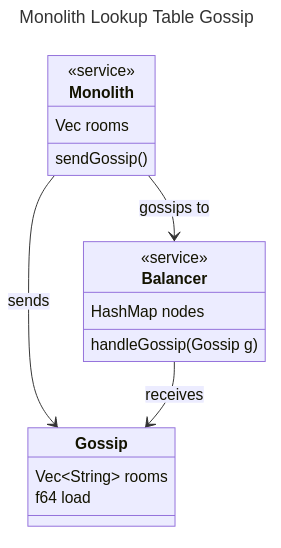
\includegraphics{Figures/gossip-class-diag.png}}
  \caption{\label{Figure::gossip-class-diag} Gossip class diagram.}
\end{figure}

\section{Creating or Loading Rooms}

The client will have three options: generating a temporary room with a uuid, creating a temporary room with inputs, and creating a permanent room that can be rejoined in the future.

The options follow similar sequence paths, as shown in figure \ref{Figure::create-room-diag}. The client starts a new Balancer connection through the websocket, then the Balancer is responsible for deciding which node is best fit to handle the additional room. Once the right one is picked, the room is instantiated on that Monolith and the client connects.

Room generation requires no inputs from the client, instead a new uuid is automatically used as the room name. On the other hand, room creation has the client submit a set of inputs for the name and settings of the room. Generation only provides temporary rooms that are discarded after the room is unloaded. Creation can provide either temporary or permanent rooms, depending on the client inputs during the initial process. The settings for permanent rooms are stored in postgres even after being unloaded so that they persist and can be called upon to be reloaded at any point in the future.

\begin{figure}[!htb]
  \centering
  \scalebox{0.57}{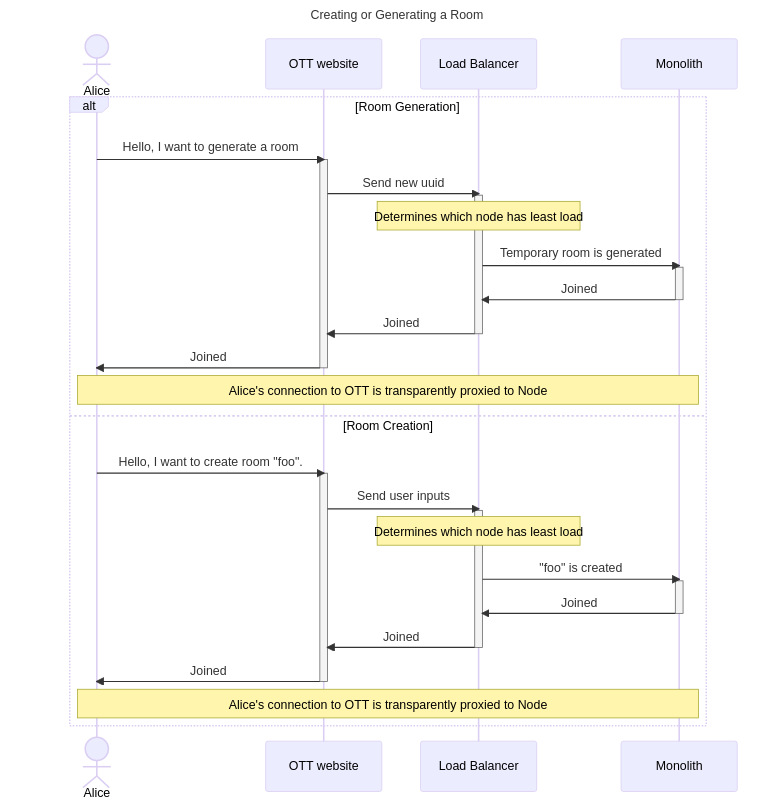
\includegraphics{Figures/create-room-diag.png}}
  \caption{\label{Figure::create-room-diag} Creating or generating a new room.}
\end{figure}

\subsection{Lifetime of a Room}

Rooms are only kept loaded in memory if there are clients that are connected to them. If a room is loaded and there are no clients connected, it will be unloaded after a certain amount of time.

\begin{figure}[!htb]
  \centering
  \scalebox{0.57}{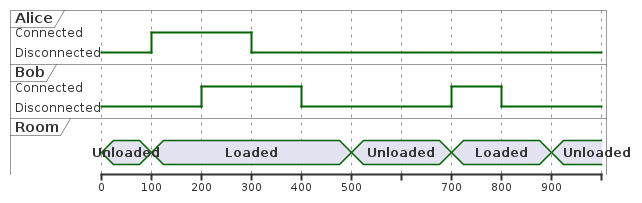
\includegraphics{Figures/room-keepalive-timing.png}}
  \caption{\label{Figure::room-keepalive-timing} A timing diagram describing the lifetime of a loaded Room in a Monolith's memory.}
\end{figure}

\subsection{Monolith Node Selection}

\subsection{Unloaded Room}
When a user tries to join a permanent room in OpenTogetherTube, the request is first received by the load balancer. 
The load balancer forwards the request to one of the available servers (Server1 or Server2) based on the current load
balancing algorithm. The selected server then checks if the requested room is already loaded by querying the database. 
If the room is already loaded, the server redirects the user to the room. Otherwise, the server requests the database to 
load the room. Once the room is loaded, the server creates a new room instance and adds it to the list of loaded rooms. 
The server then redirects the user to the loaded room through the load balancer. If the first server doesn't have the
room loaded, the load balancer forwards the request to the second server and the same process is repeated.

\begin{figure}[!htb]
  \centering
  \scalebox{0.57}{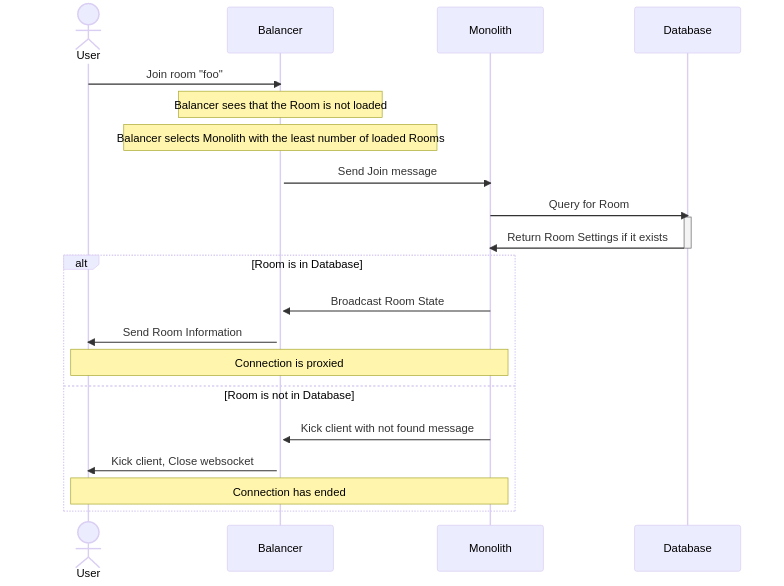
\includegraphics{Figures/unloaded-room.png}}
  \caption{\label{Figure::unloaded-room} Unloaded Room Sequence Diagram.}
\end{figure}

For the sequence diagram above, it's worth noting that the current implementation doesn't necessarily use an HTTP
redirect to direct the user to the requested room. Instead, the response from the server may include a URL or other
information that allows the user's client to connect directly to the appropriate room instance.